\chapter{Methods: Multilevel Analysis and Corpus Linguistics}
\lhead{\textit{Methods: Multilevel Analysis and Corpus Linguistics}}

\textit{\textbf{Chapter Summary:} This chapter introduces a multilevel discourse methodology. The levels (ecological, cultural, socio-economic, and cognitive) arise from past and current junctures in intercultural communication research. Three levels of communication are also proposed: textual, verbal, and non-verbal. Corpus linguistics is then introduced as a way to apply the multilevel methods to real world linguistic data.}
\newline

The research question at hand relates to both intercultural communication and the natural environment. It is, therefore, necessary to employ a methodology suitable for both of these themes. Obviously, this is an ambitious task since these are each very complex and expansive subject areas.    

The literature review in Chapter 1 stresses the need for interdisciplinary, holistic approaches. From the social scientific standpoint, existing methodologies in intercultural communication research provide such interdisciplinary, holistic frameworks. Recognizing that studying culture and communication is an exercise of grappling with complexity, ICC research has evolved from simple, essentialized values to ``complex theorizing and modelling'' \citep[186]{Oetzel2007a}. In other words, research has acknowledged that a synthesis and integration of factors is necessary in order to understand cultural interactions. To integrate the many levels and contexts . However, these approaches have often been employed for social scientific inquiry. In the current study, the challenge is formulating a \textit{multilevel} method that accounts for both social and natural phenomena.  

A preliminary question for multilevel analysis is which parts or `levels' to take into account. For instance, Brofenbrenner's socio-ecological framework for human development proceeds from the individual to the micro, macro, exo, and macro systems. Various social relationships and institutions correspond to the levels; for example, family is within the micro-system while one's culture is the macro-system. By contrast, models employing systems theory might identify key variables. Biophysical or technical systems, for instance, often begin with inputs/outputs. 

To determine which levels to consider in intercultural interactions, we can look to historical developments within ICC as a field. Since intercultural communication research formally began over a half-century ago, various levels have been investigated. Broadly speaking, there was a micro-cultural emphasis beginning in the 1950s and 60s, which was followed by a critical turn in the 80s and 90s. The former looked at the details of everyday communicative interactions, while the latter gave greater consideration to external factors (social, political, economic). More recent calls for an ecological turn in intercultural communication studies could be characterized as a further continuation of this external, macro-contextual focus.

In what follows, we develop levels of analysis by considering the history of ICC research. It is argued that what are now called the cognitive sciences influenced early ICC research and remain crucial to the field. Accordingly, we propose cognition as the micro-level of analysis. In response to recent calls for an ecological turn in the field, ecology is suggested as a macro-level of analysis. It is argued that ICC has yet to integrate micro/macro approaches and that multilevel analysis is a possibility for doing so. 

\section{Levels of ICC Research}

As a discipline, intercultural communication emerged in the post-WWII era when the Foreign Service Institute (FSI) hired linguists and anthropologists to develop ``pre-departure courses'' for US diplomats and personnel \citep[4546]{LeedsHurwitz2013a, Martin2010a}. From these early stages, intercultural communication focused on face-to-face, situated, and nonverbal communication. \cite*{Hall1966a} developed proxemics as the study of ``social and personal space'' in interpersonal interactions (1). \cite*{Birdwhistell1952a} developed kinesics to interpret expressions, gestures, and body movements in communication. The term paralanguage was introduced by \cite*{Trager1958a} to refer to voice modification in utterances. This early emphasis on nonverbal, non-symbolic communication contrasted with then-prominent sender-receiver models of information transfer \citep[e.g.,][]{Shannon1949}.

During the same years that linguists and anthropologists were laying the groundwork for intercultural communication, a more theoretical interchange was taking place between anthropology and linguistics as well as psychology and the then-emerging fields of artificial intelligence, computer science, and neuroscience. In what would later be called the \textit{cognitive revolution}, researchers in several fields began to develop theories of mind and intelligence. Notably, \cite*{Miller1956a} proposed that limitations of working memory were overcome by chunking information; \cite*{Chomsky1959a} rejected behaviorist approaches to language in favour of the notion of mental grammars; \cite*{Newell1958a} advanced a theory of human problem solving in terms of elementary information processes. These researchers, together with pioneers in artificial intelligence such as McCarthy and Minsky, gave rise to the field of cognitive science \citep{Thagard2018a}.

It could be argued that, in the early stages of ICC as a discipline, researchers at the FSI were also thinking of culture in terms of mental states and cognition. By considering cultural aspects of communication, intercultural research was\textemdash at least implicitly\textemdash adopting cognitive assumptions about the relation between language and thought. Apparent in the work of Trager, Hall, and other FSI researchers is the notion that linguistic meaning arises not only from words but from a combination of ``metalinguistic'' levels \citep{LeedsHurwitz2013a}. These levels\textemdash exhibited through micro-cultural behaviors and nonverbal interactions\textemdash were understood as culturally relative. Crucially, cultural variations were attributed differing conceptual schema. Accordingly, obtaining an understanding of another culture is analogous to developing a theory of mind; that is, it requires the ability to impute mental states to others \citep{Premack1978a}. In \textit{The Silent Language}, \cite*{Hall1958a} speaks of the challenge of ``achieving understanding and insight into mental processes of others'' (52). Later he refers to cultural understanding as gaining insight into the ``cognitive world'' \citep[155]{Hall1966a}.

This is not to suggest that links between cognitive science and intercultural communication were explicit. These links are more likely a reflection of shared intellectual antecedents in anthropology and linguistics at the time. Influences on Hall and other FSI researchers included Frank Boas whose work on sense and perception would later lead to cognitive anthropology \citep[2021]{Colby1996a, Cole2013a, Shore1996a}. Also influential was linguistic relativity (Sapir-Whorf hypothesis) and the view that language influenced conceptual and cognitive domains. In fact, Hall's (\citeyear{Hall1966a}) thesis in \textit{The Hidden Dimension} is that ``principles laid down by Whorf'' apply to ``all culture'' (2). In addition to these intellectual antecedents, one might also consider that the specific interdisciplinary challenges FSI researchers were addressing may have led to cognition as a fundamental consideration. Whereas the siloed study of anthropology and linguistics lends itself to descriptive, etic approaches, the practical challenges of intercultural interaction entail reapproaching both culture and communication in terms of the mind and conceptual schema.

Despite the cognitive thrust of early ICC research, the notion of culture as something internal to the mind was perhaps too limited to take hold in a discipline that needs to account for multilevel, societal interactions. Cognitivist views of the mind downplay the social and environmental factors that influence mental processes. From early symbolic AI to connectionist approaches beginning in the 1980s, cognitive functions have been conceptualized in an internal manner through computational metaphors. Arguably, cognitivist approaches to the mind led to overly reductive understandings of human communication and culture. Nonetheless, sub-disciplines of cognitive science went on to make contributions highly relevant to intercultural communication. Social cognition, for instance, emerged from psychology in the 1970s and led to research into perception, categorization, and stereotype \citep{Augoustinos1995a}. However, interest in how culture influences social cognition has been relatively recent \citep[e.g.,][]{Aronson2010}. In other words, there has not been an approach to studying the mind that fits the macrocontext of intercultural communication; that is, one that considers interactions between society, cognition, communication, and culture.

Beginning in the 1980s, intercultural communication research began to be influenced by rise of postmodernism and social constructionism within the social sciences. These trends gave way to the critical turn in the 1990s. This was a turn away from microanalytic, essentialist approaches to culture, towards critiques of power, oppression, and structural political/economic inequalities \citep{Moon2011a, Halualani2009a}. In essence, the critical turn was a movement towards the macrocontext.

While the critical turn expanded the scope of intercultural communication research, this may have been at the cost of cognitive approaches laid out in earlier decades. Critical intercultural communication scholarship developed in a way that often precluded multilevel interactions involving cognition. Despite the interdisciplinary emphasis, scholars in critical theory and cultural studies showed minimal interest in cognitive science \citep[123]{Crane1999a}. It could be argued that, by viewing meaning as developed discursively with others, social constructionism downplays the role of cognition and the mind \citep[2]{Bondebjerg2017a}. 

To this day, it remains relatively uncommon in ICC research to focus on cognition. Searching the \textit{Journal of Intercultural Communication Research} and \textit{Language and Intercultural Communication} for articles with titles or keywords containing ``cognitive'' or ``cognition'' yields only 3 and 2 results respectively. Although these results are less than one might expect given the extent of disciplinary overlap, the finding is unsurprising if we consider the scope and trajectory of ICC in the last half of the 20\textsuperscript{th} century.

\subsection{The Ecological Turn}

Although critical intercultural communication integrated the broader social context, both culture and communication remained conceptualized in the human realm. In other words, the ecological context remained an anomaly. Recognizing the human-centered focus of critical research, \cite*{Mendoza2016a} have recently made the case for an ``ecological turn'' in intercultural communication. On the surface, this turn is a further development towards the macrocontext. The ecological context also highlights the need for multilevel analysis.

\cite*{Mendoza2016a} re-examine key assumptions of intercultural communication by employing ethnoautobiography, a methodology meant to connect to ``place, history..., nature, spirit, ancestry (indigenous origins), and community'' (4). Expanding on the notion of an ecological turn, \cite*{Kinefuchi2018a} proposes critical discourse analysis (CDA), a methodology that examines power, ideology, and social-structural forces. Kinefuchi also draws attention to CDA as a method for ``analyzing the relationship between macrocontext and microinteraction'' (213). The focus on both the human subject (through ethnoautobiography) as well as the macrocontext (through CDA) implies the ecological turn requires the study of multilevel interactions. Levels range from the human subject to social-structural factors and beyond, to the natural world. Although difficult in practice, multilevel analysis is necessary to capture the complex relationship between humans and the natural world. 	

Kinefuchi's adoption of CDA as a methodological approach for an ecological turn invokes the critical tradition, since CDA falls squarely within the critical turn in ICC. In other words, CDA addresses the social and political context, but it is not clear how it encompasses other factors. A multilevel approach entails a broader scope for discourse analysis encompassing the cognitive, social, cultural, and ecological levels. Even though variants of CDA take these levels into account, its origins and focus lie in the social realm. The application of CDA to ecology raises the question of whether discourses related to human-caused environmental issues (such as species loss, climate change, and pollution) can be understood and analyzed in the same way as social issues (such as inequality, oppression, racism). Similarly, applying discourse analysis to culture and cognition requires moving beyond the socio-economic critique characteristic of CDA. 

\section{Multilevel Discourse Analysis}

The previous section outlined how ICC research has ranged from microanalysis and mental states; to the critical analysis of socio-economic factors; and, finally, a more recent turn to the ecological context. The present challenge is the integration of approaches. This dissertation draws on discourse analysis as a methodology for analyzing human communication. However, rather than an exclusive focus on critical discourse analysis (CDA), a type of multilevel discourse analysis is proposed.

The term \textit{multilevel analysis} is not new. Multilevel discourse analysis (MDA) is commonly associated with \cite*{Fairclough1992, N.2003} as a method to examine  multiple levels of texts. These levels refer to language within texts (intratextual), between texts (intertextual), as well as the broader historical context (contextual). In CDA frameworks, multilevel has also been used to refer to mediation between the linguistic (textual) and sociopolitical context with a \textit{meso} level of human action and cognition \citep[e.g.,][]{Trimithiotis2018}. The term multilevel is also used beyond discourse analysis. For instance, in management literature, multilevel is implied when there distinction is made between macro and micro \citep[e.g.,][]{Bitektine2014}. Multilevel is also used in statistical modeling or, more generally, any situation involving units at a lower (micro) level nested within units at a higher (macro) level \citep{DiezRoux2002}.   

The multilevel discourse analysis proposed in this dissertation integrates the levels of intercultural communication research which were discussed in the previous section. The higher (macro) level is the ecological context, as indicated by the ecological turn in ICC. The lower (micro) level is cognition, such as the emphasis on mental states charactersitic of early ICC research. As explained below, the \textit{meso} levels in this framework are cultural and socio-economic. Thus, the proposed multilevel framework includes four levels of analysis: (i) ecological; (ii) cultural; (iii) socio-economic; and (iv) cognitive (Figure 2.1).

\begin{figure}[H]
\centering
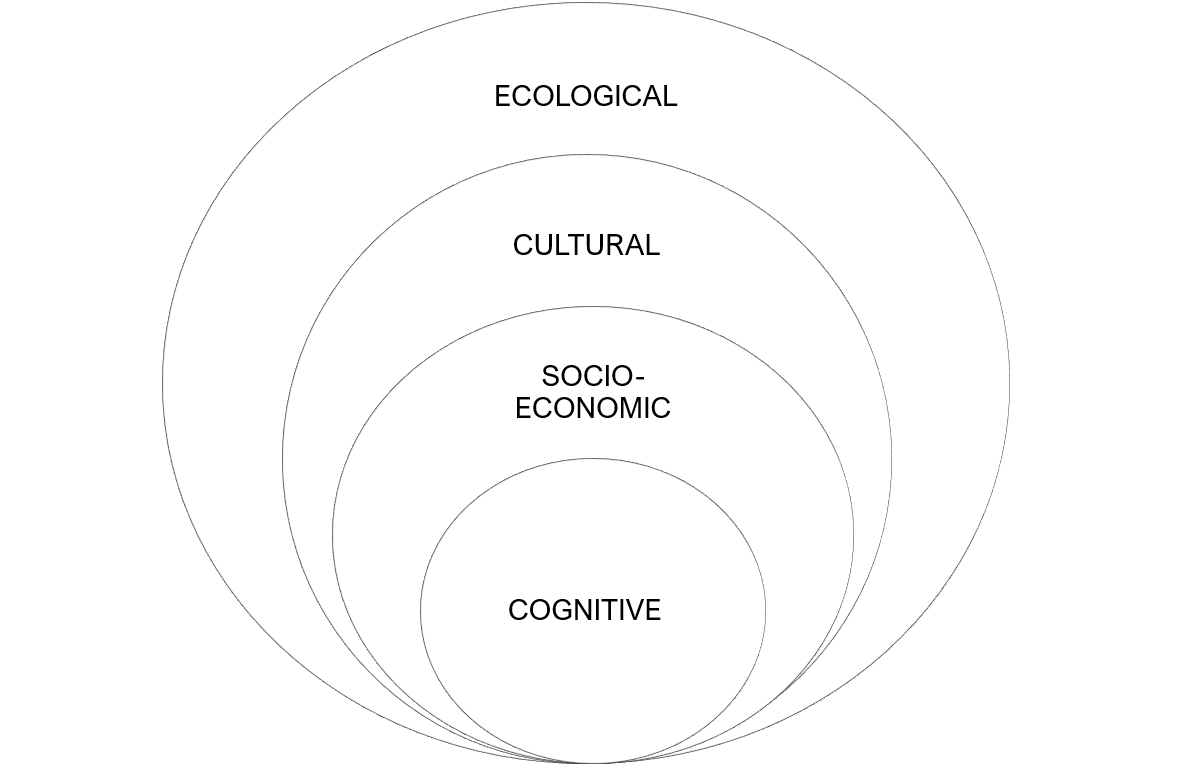
\includegraphics[width=8cm]{Figures/nested.png}
\caption{Levels of discourse analysis proceeding from the ecological macro-context of natural systems, to the micro-context of cognition}
\label{fig:figure1}
\end{figure} 

Discourse analysis is employed to gain insights into communication within and between the levels. These insights might include rhetorical styles, linguistic devices, power relations, ideologies, biases, identities, and other phenomena that may not be apparent on the surface of communication. Discourse analysis is concerned with naturally occurring language beyond standard linguistic units of analysis (i.e. morphology, semantics, and syntax). The `larger' units of interest to discourse analysis include texts, conversations, speech acts, or other communication events. The term discourse can apply to a broad range of communication. It primarily refers to language-in-use \citep{Wetherell2001}, but might also extend to nonlinguistic or multimodal communication including gestures, film, media, art, and sound \citep[2, 15]{Wodak2009}. 

In the sections that follow, each of the levels is outlined, with examples. Discourse is categorized under a given level primarily based on the semantic content. However, the extra-linguistic context is also important. Each level has two main elements: (i) the \textit{data} which refers to the communication itself; and (ii) \textit{analysis} of that data. 

\subsection{Ecological Level}

In the simplest terms, the ecological level refers to discourse about the natural world or the environment [\textit{Umwelt}]. This could obviously cover a wide range of communication, encompassing scientific statements or, outside of formal science, statements about the more-than-human world. The ecological level follows from the formal definition of ecology as a ``branch of biology dealing with the relations and interactions between organisms and their environment.''\footnote{https://www.dictionary.com/browse/ecology} In addition, the ecological level is concerned with human subjective experiences of the natural world and their surroundings. For instance, the present use of the term ecology also accounts for Jakob von Uexk\"ull's (\citeyear{VonUexkull1982}) semiotic concept of \textit{Umwelt}, which refers to the environment as the organism's centre of communication and signification rather than biophysical flows of material and energy (as in the strictly natural scientific concept of the environment). In other words, the \textit{Umwelt}, as experienced by the human subject, is the source of signification and meaning not only for the individual subject, but that is shared (intersubjectivity).

To illustrate what communication would be considered ``ecological,'' consider both of the following statements:

\begin{footnotesize}
\begin{itemize}
    \item[-] \texttt{Biodiversity has declined 27 percent in the last three decades.}
    \item[-] \texttt{I love to walk in the forest.}
\end{itemize}
\end{footnotesize}

The first statement is an empirical assertion that falls within the formal study of ecology. The second relates to a subjective experience of the natural world. In the present discourse analytic framework, both statements would be considered as part of the ecological level. The analysis of the statements would depend on the context. For example, if the above statements were placed in the following contexts, their interpretation would change considerably:

\begin{footnotesize}
\begin{itemize}
    \item[-] \texttt{Biodiversity has declined 27 percent in the last three decades, which justifies the total overhaul of our political and economic system.}
    \item[-] \texttt{I love to walk in the forest...experiencing nature is part of my identity and values as someone from rural Vermont.}
\end{itemize}
\end{footnotesize}

These contexts demonstrate how the levels are not distinct; rather, they often blend together. As discussed in later sections, the first statement would be analyzed with the socio-economic level while the second would be considered cultural.  

The ecological level obviously relates to natural sciences and scientific communication. It should be stressed, however, that the present study does not aim to employ methods of the natural sciences and, accordingly, the ecological level of analysis is not intended as scientific analysis. In line with critical science studies, scientific discourse is viewed in a social and cultural context, as having a semiotic role. Thus, the ecological level of analysis aims to bridge the social/human and natural sciences while maintaining critical, meaning-centred analysis. Such an aim is consistent with that found in political ecology literature. \cite*{Escobar1999}, for instance, refers to ``a new articulation of the natural and human sciences'' where the ecological realm is ``understood in biological terms but [also] in complex relation with cultural and economic practices'' (15). Along the same lines, \cite*{Peet2011} see natural sciences as ``essential to solving environmental problems'' but also as ``historically problematic parts of those problems'' (31). The aim is to employ a critical humanistic framework that challenges the so-called objective position of the natural sciences, but also accepts the crucial role for the scientific method in understanding and addressing ecological issues. 

To summarize, the ecological level \textit{data} consists of communication about the environment which often includes, but is not limited to, scientific communication. Ecological-level \textit{analysis} of that data is concerned with the social, cultural, and semiotic dimensions of ecological communication.

\subsection{Cultural Level}

A challenge for intercultural communication research is the very meaning of `culture'. In 1871, the anthropologist Edward Tylor offered a broad definition of culture as ``that complex whole which includes knowledge, belief, art, law, morals, custom, and any other capabilities and habits acquired by man as a member of society'' \citep[1]{Tylor1871a}. Ever since, scholars have been attempting to add specificity to Tylor's definition, focusing on external artefacts and behaviour; symbolic meanings; or psychological dimensions \citep[see][for an overview]{Prinz2016b}. To this day, there is a ``lack of clarity and consensus'' concerning culture \citep[12]{Minkov2013a}. The widespread use of the term, together with its ambiguity, has led some to dismiss scientific use of the concept altogether \citep[e.g.,][]{Barber2008a}. 

\cite*{Blommaert2005a} asserts that it does not make sense to speak of ``noncultural'' discourse (4). This statement reflects the notion that culture is ubiquitous \citep[15]{Neuliep2018a} or ``everywhere'' \citep{Hannerz1993a}. Given this sweeping scope, the question for a multilevel approach is how to distinguish culture from other levels. Since a potential drawback of multilevel research is its broad scope \citep{KleinK.J.TosiH.&Cannella1999a}, it is particularly important to avoid compounding this drawback through an overly broad view of the term culture. An overly broad view could, for example, lead one to characterize misunderstandings as intercultural when economic, political, or other social factors would provide a more accurate and descriptive account. In the opening chapter, for example, the failure of global climate change policy is discussed as one such example where political and economic factors are more likely at play than cultural differences. In order to analyze such complex issues, we can aim to delimit culture from other levels of social interaction.

To study how culture is reflected in discourse, various frameworks have been proposed including ``cultural discourse analysis'' \citep{Carbaugh2007a} and ``cultural approaches to discourse'' \citep{Shi-xu2005a}. Cultural discourse analysis (CuDA) draws out the ``symbolic meanings'' and ``cultural commentary'' that pervade human communication \citep[168]{Carbaugh2007a}. Other methods related to the cultural aspects of communication include ethnography of communication \citep{Hymes1972a} and speech codes theory \citep{Philipsen1997a}.

For the present multilevel framework, the cultural level refers to when people are expressing or commenting on who they are. Cultural discourse generally reflects one's identity, values, or worldviews. For instance, the following are some examples of statements that would fall into the cultural level of analysis.

\begin{footnotesize}
\begin{itemize}
    \item[-] \texttt{This is my home, and I will protect it.}
    \item[-] \texttt{God will take care of us.}
    \item[-] \texttt{Our ancestors would be proud.}
    \item[-] \texttt{I am American but France is my real home.}
\end{itemize}
\end{footnotesize}

Whether a statement is cultural will often depend on who the speaker is and how they identify as a member of a group. For instance, if speakers refer to themselves with a cultural or ethnolinguistic identity, then it is more likely that their words are expressing something with cultural significance. For instance, the following quote shows cultural self-identification.

\begin{footnotesize}
\begin{itemize}
    \item[-] \texttt{As indigenous women, we are here to protect our community.}
\end{itemize}
\end{footnotesize}

The above example contrasts with cases where an identity is assigned to another in the discourse, such as in the following statement:

\begin{footnotesize}
\begin{itemize}
    \item[-] \texttt{The protestors, who were mostly migrants from Mexico, were unruly.}
\end{itemize}
\end{footnotesize}

Here, the national/cultural identity \textit{Mexican} is assigned by the narrator. Such cases might still be considered cultural-level discourse, but likely with more critical analysis of the assigned identity. For instance, the cognitive dimension of stereotype might come into play in the analysis of this statement.

To summarize the cultural level, \textit{data} consists of communication that expresses meaning or identity in some way. The nonverbal component of the cultural level is also important, as speech style, gesture, and dress are all important elements of culture. \textit{Analysis} at this level asks how culture is being expressed, or what worldviews are implicit in the communication. At the cultural level we are cognizant of how identities are assigned. Being wary of stereotype and othering is crucial in this level of analysis.

\subsection{Socio-Economic Level}

The socio-economic level relates to what has typically been the focus of Critical Discourse Analysis (CDA). CDA is generally concerned with how social power relations are established and reinforced through language \citep{Fairclough1995}. Central to CDA are explicit or implicit goals of social change, which presuppose certain shared notions of justice, equality and `the good'. Critical analysis aims to expose and resist oppressive economic, social, and political structures that are enacted and perpetuated through language and communication. Beginning with the critical turn in the 1990s, CDA influenced critical intercultural communication \citep{Moon2011a}. 

The current multilevel framework\textemdash while maintaining an emphasis on critical analysis\textemdash distinguishes between the cultural and social realms. The social-level encompasses statements about economics, institutions, laws, and power relations. The following are examples of statements that would fall into the social level:     

\begin{footnotesize}
\begin{itemize}
    \item[-] \texttt{Unemployment in the community is higher than the national average.}
    \item[-] \texttt{Government and policy makers are only there to protect corporations.}
    \item[-] \texttt{The police used excessive force.}
\end{itemize}
\end{footnotesize}



\subsection{Cognitive Level} 

While many discourse analytic approaches study the relations between society, culture, and discourse, a socio-cognitive approach considers these relations as mediated by cognition \citep[64]{VanDijk2015a}. Attitudes, ideologies, and beliefs stem from cognitive structures that constitute social and cultural relations through discourse. Analogously, discourse establishes and reinforces cognitive structures. This link opens possibilities for intercultural communication research that is engaged with cognitive science while, at the same time, maintaining a social-critical edge. Here, we define the cognitive level of discourse as communication that provides insight into mental processes, particularly the unconscious. Cognitive level \textit{data} is any communication that provides these insights, while the \textit{analysis} seeks to arrive at the insights themselves. In other words, cognitive analysis establishes the relation between communication and mental representations. 

The cognitive level draws on concepts from cognitive linguistics. These concepts, which are developed in more detail in subsequent chapters, include the following:

\begin{itemize}
    \item \textit{Conceptual metaphor}: the understanding of one idea, or conceptual domain, in terms of another; a mapping between conceptual frames \citep{Lakoff1980a}. 
    \item \textit{Implicature}: inferential and context dependent knowledge domains or mental schema \citep{Grice1975}.
    \item \textit{Conceptual Blending}: how the combining and mapping of concepts gives rise to meaning as an emergent structure beyond the sum of its parts \citep[403]{Evans2006a}
    \item \textit{Idealized Cognitive Models}: the background knowledge that structures our mental spaces \citep{Lakoff1987}.
    \item \textit{Stereotype and othering}: categorizations that help to simplify and organize information, often manifesting as in-group/out-group generalizations \citep{Tajfel1981}.
    \item \textit{Nonverbals \& Emotions}: gestures, facial expressions, paralanguage and other nonverbals as a reflection of unconscious cognitive processes. 
\end{itemize}

Cognitive analysis plays an important role in understanding and interpreting communication beyond explicit written or spoken words. The other three levels of analysis rely more on explicit semantic content of utterances. The cognitive level, by contrast, relies more on implicit context, linguistic devices, and nonverbal expressions.

Cognitive level \textit{data} would be excerpts or examples of communication that demonstrate cognitive concepts, such as metaphor, implicature, blending, etc. Data also consist of visual and multimodal communication that permit the analysis of nonverbal communication. \textit{Analysis} relates to the interpretation of the data as well as insights concerning how cognition may be the basis of communicative misunderstandings.   

\subsection{Summary of Levels}

The four levels are summarized in Table 2.1 below. To separate levels in this way is, of course, a simplification. In reality, these factors blend together and there are not clear dividing lines between them. Ecological discourse is often cultural, the cultural and social realms are overlapping, and so on. Likewise, insights from cognitive linguistics do not apply to a subset of communication, they are features of communication itself. Nonetheless, in segmenting communication in this way, we are interested in prototypical examples of each level. Accordingly, we can better analyze each level and, ultimately, understand how the various levels interact.

\begin{table}[H]
\begin{footnotesize}
\centering
\def\arraystretch{1.5}% 
\begin{tabular}{ | P{4cm}| P{5.75cm} | }  
 \hline
\textbf{Level} & \textbf{Description} \\
 \hline
\textbf{Ecological} & Discourse about nature and the more-than-human world; includes discourse that concerns ecology in a scientific sense, as well as human subjective experiences (\textit{Umwelten}) \\
 \hline
\textbf{Cultural} & Expressions of identity, values, and worldviews; people commenting about who they are, either directly or indirectly  \\
 \hline
\textbf{Socio-Economic} &  Discourse related to economics, institutions, and power relations; aspects of social existence that do not express cultural identity \\
 \hline
\textbf{Cognitive} & Mental representations and cognitive frames as reflected in communication; drawing on concepts from cognitive linguistics as well as nonverbal communication \\
 \hline
\end{tabular}
\caption{Summary of levels of discourse}
\label{tab:table1}
\end{footnotesize}
\end{table}

\subsection{Levels of Communication Data}

Thus far, we've discussed levels as themes (ecological, cultural, socio-economic, and cognitive) to group the data and analysis. In addition to these four thematic levels, there are also multiple linguistic/communication levels, which relate to the type of data that is gathered. For example, in discourse analysis, one would consider different modes of communication such as texts, speech, body language, etc. Although discourse analysis has traditionally focused on the textual level, the term \textit{discourse} can encompass diverse forms and modalities of human communication.

For this study, communication data is segmented into three levels as outlined in Figure 2.2: (i) the textual level of written communication; (ii) the verbal level of spoken (lexical) communication; and (iii) the nonverbal level of spoken (non-lexical) communication. Like the thematic levels, these levels of communication are hierarchically ordered from general to specific, or from the macro- to micro-context. Multimodal communication is the blending of the three levels and is more representative of communication in real life.

\begin{figure}[H]
\centering
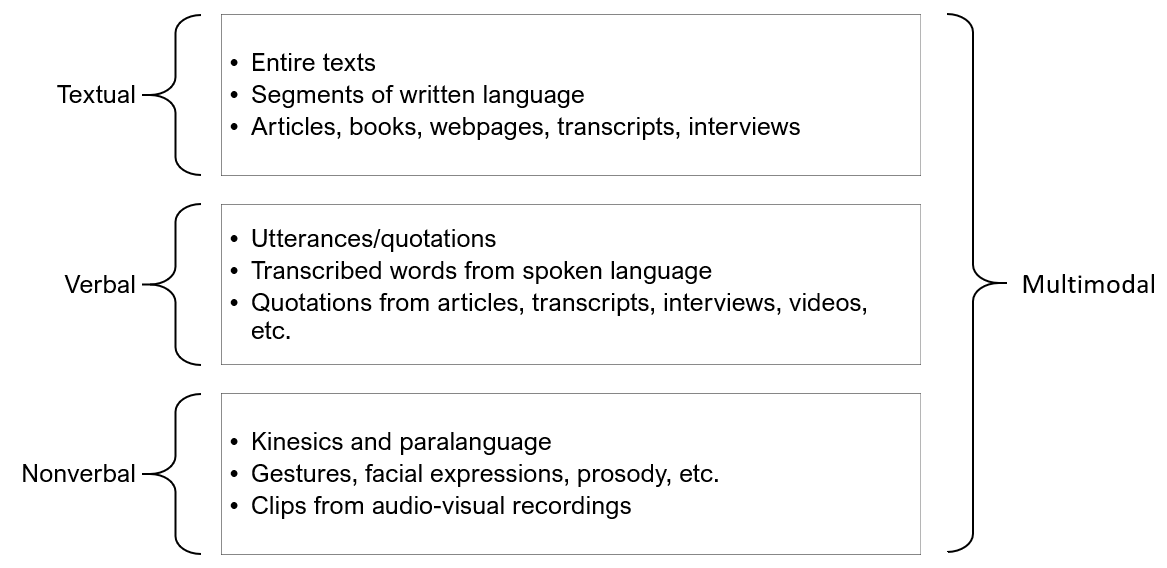
\includegraphics[width=12cm]{Figures/levelscomm.png}
\caption{Levels of communication with examples of data}
\label{fig:figure1}
\end{figure}

The \textbf{textual level} is concerned with entire texts and segments of language beyond utterances and sentences. Objects of textual analysis include articles, book excerpts, webpages, transcripts, and interviews. Of interest at this first level are broad themes, keywords, and rhetorical styles. The \textbf{verbal level} concerns utterances or statements made my a specific individual or possibly a group (e.g. group chants, slogans, etc.). In addition to their original source, utterances are obtainable from quotations in articles, transcripts, videos, or interview segments. As with the textual level, themes, keywords, and style are all of interest and serve as context for analysis. However, what distinguishes the verbal from the textual level is the identity of the speaker. Whereas textual data abstracts the speaker away from the text, the verbal level links utterances to a specific speaker. Finally, the \textbf{nonverbal level} considers nonlinguistic communication which may be visual, auditory, tactile, or kinesthetic. Gestures, facial expressions, pitch, and intonation are all examples of nonlexical components that are essential to meaning.

Of course, as with the thematic levels, textual, verbal, and nonverbal communication are not entirely separable in the flow of everyday life. Meaning and understanding arise from the interactions of these elements into multimodal, semiotic events. However, organizing data and analysis in a way that isolates the various elements allows for the investigation of the otherwise overly complex phenomena of human communication.

\section{Corpus Linguistics}

Above, we introduced four levels of analysis related to themes of discourse as well as three levels of communication data. This section addresses the data collection itself; that is, how we obtain representative samples of data that cover the levels and from which meaningful insights can be drawn.

When it comes to data collection, some trade-offs have to be made. As alluded to above, the very notion of communication as ``data'' is a simplification in that holistic semiotic events in the \textit{Lebenswelt} are categorized and isolated in order to be studied. Yet, to study a phenomena in a systematic way, we often need to move away from holistic communicative events and towards analyzable components. To decontextualize and reduce communication in this way simplifies complex phenomena. What's gained from this simplification, however, is generality and the ability to draw insights from a broad range of communicative situations. By employing different modes of inquiry (both qualitative and quantitative) the present methodology aims to strike a balance in a way that leads to generalizable conclusions while appreciating the complexities and nuances of communication and culture. 

This section introduces corpus-based approaches to both ecological and intercultural communication. Based on the lack of existing corpora in these areas, the case for custom, specialized corpora is made. Corpora constructed specifically for the present research problem are then discussed, in addition to how they are analyzed in subsequent chapters.

\subsection{The Need for Data Volume \& Variety}

To gain meaningful insights, data must be collected and patterns observed across a variety of situations and settings. In other words, a large volume and variety of communication needs to be analyzed. A multilevel approach only adds to these data requirements. To carry out ecological, cultural, social, and cognitive analyses requires data covering a wide range of themes and subject matter. Likewise, we need a combination of textual, verbal, and nonverbal data. A key methodological criterion, therefore, is the ability to gather and analyze a sufficient variety and volume of real human communication.

For the research question at hand, many common methods of intercultural communication research would be insufficient in terms of meeting the data requirements. These methods include ethnography of communication, interpretive interviews, postcolonial ethnography, and critical discourse analysis \citep{Oetzel2016a}. Ethnography of communication often requires extensive field work, which limits the geographic and temporal scope. Face-to-face interpretive interviews have similar scope limitations. While these and similar methods (involving primary-source data collection) are essential for a first-hand understanding of cultural and communicative events, they often limit the amount of data that can be collected. By drawing from secondary sources, CDA and other discourse analytic approaches allow for more data volume, but are still limited by the amount of linguistic data the researcher can read and interpret. Discourse-based methods often emphasize qualitative analysis through close reading of texts as well as interpretation of the extra-linguistic context. With this emphasis comes obvious limits to the amount of text a researcher can qualitatively assess. 

\subsection{Corpus Linguistics to Address the Data Challenge}

Ideally, a methodology would combine the emic depth of ethnographic field studies with the breadth and generality possible with large and varied data sets. However, these two aims are often inversely related. To strike a methodological balance, the present study proposes corpus linguistic methods for data collection and analysis. Corpus linguistics is one way to meet requirement for large data sets. In linguistics, a corpus is a collection of machine-readable texts stored in an electronic database \citep[48]{Baker2006c}. While a corpus does not contain new information, computer aided analysis can offer ``a new perspective on the familiar'' or insights that would be impossible through human analysis alone \citep[2-3]{Hunston2002a}. As \cite*{Belcher2013a} point out, digital corpora allow for a ``breadth or sheer numbers of texts and depth of analysis'' beyond what an individual could achieve ``despite their linguistic expertise and emic/etic cultural perspectives'' (1).

Several previous studies have effectively used corpora for discourse analysis. Large bodies of text allow for objective, quantitative approaches, adding to the generality and confidence of findings \citep[e.g.,][297]{Gabrielatos2008a}. These advantages are particularly pertinent given that a common criticism against CDA is that researchers can ``cherry-pick'' data samples based on their aims and assumptions \citep{Mautner2009a}. Although corpus approaches to discourse analysis have increased in recent years, applying corpus linguistics to either environmental or intercultural communication is even more recent and there are still relatively few corpus-based studies in these fields. 	

The methodological aim in this dissertation is to use corpus methods to study intercultural environmental communication. This aim leads to several questions pertaining to the size, balance, and representativeness of corpora which could be used for this purpose. A key question is whether existing corpora might be suitable or if new ones are required. Before addressing these questions, however, some more background is required regarding corpus linguistic approaches to both ecological and ICC research.

\subsection{Corpus Linguistics \& Ecology}

To consider how corpus linguistics might be applied to ecological questions we can look to the nascent field of ecolinguistics. Ecolinguistics is often traced to Haugen's (\citeyear{Haugen1972a}) introduction of the ``ecology of language'' as ``the study of interactions between any given language and its environment'' (325). Ecolinguistics became more prominent in the 1990s and was explicitly linked with modern environmentalism by \cite*{Halliday2001a}, who drew connections between ``linguistic anthropocentrism'' and unsustainable growth. As a relatively new, evolving approach to both linguistic and ecological research, the precise definition and scope of ecolinguistics remains open to interpretation. Some emphasize a metaphorical understanding of language as a living system, while others are more concerned with discourses that lead to environmental degradation \citep[see][for an overview]{Chen2016a}. An ecological approach to language raises a number of conceptual questions such as what constitutes the ecological context of language, or whether the relation between language and the physical environment is bidirectional or unidirectional \citep{DoCouto2014a}. Notwithstanding these challenges, ecolinguistics has emerged as an important interdisciplinary approach to both environmental and linguistic research. 

Although corpus methods have been effectively applied to ecolinguistic questions \citep[e.g.,][]{Poole2016a, Poole2018, Stibbe2003a}, there are many unexplored research questions suited to corpus approaches. Many of these questions carry over from existing areas of linguistic inquiry \citep[see][]{Cheng2012a}. For example, questions might concern new uses and meanings of words. As with other regions of language, words related to nature, landscapes, or species are continuously evolving. Consider the term ``wetland'' which was adopted to euphemistically replace ``swamp'' and came into scientific use in the latter half of the twentieth century \citep{NationalResearchCouncil1995}. Corpus approaches could provide insight into the evolution of such terms, including the historical and cultural factors surrounding use changes. In addition, even though the term has important legal implications, there is ambiguity regarding what exactly constitutes a wetland. There is, therefore, a role for corpus research in understanding the diverse uses of ecological terms by different groups.

Ecolinguistic research also investigates how grammar or lexical semantics construe the natural world in certain ways or possess anthropocentric properties. The passive voice, for instance, might be used to avoid human agency and responsibility \citep{Kahn2001a}. The use of pronouns (e.g. relative, personal, and possessive) in reference to nonhuman animals might also provide insight into human attitudes and behaviors towards other species \citep{Gilquin2006a}. The contextual meaning of lexical items will also frame and reflect the human relation to other species. \cite{Stibbe2003a}, for instance, refers to the British National Corpus (BNC) to demonstrate how pigs have overwhelmingly negative connotations compared with other animals. Grammar and semantics may also reveal taken for granted worldviews or ideologies that have profound environmental consequences. \cite*{Halliday2001a} points out how use patterns of forms of the word ``grow'' (e.g. growth, growing) reveal how ``deeply emgrammatized'' growth is in modern language and culture. The cross-linguistic study of lexical semantics could also provide insight into different meanings and cultural linguistic constructions of the natural world. For example, it has been argued that pronoun drop in certain languages (e.g. Japanese) may moderate individualism and perhaps even affect the environment-culture relationship \citep{Kashima2003a}. 

Ecolinguistic questions can also be investigated through inquiries into genre analysis, professional communication, or media discourse. For instance, assembling a specialized corpus of Environmental Impact Assessments (EIA) or other regulatory processes would enable comprehensive analysis of this genre of communication which is the standard in development and land use change. Along these lines, \cite{Sousa2012} applied corpus methods to regional planning rhetoric, concluding that there was a discourse orientation towards development rather than conservation. As environmental issues have become global and mainstream, critical approaches might analyze stereotyping and bias in environmental discourses \citep{Muhlhausler2006b}. Analysis of political or corporate discourses might also address the framing of environmental issues, power relations, and other themes related to political ecology and environmental justice. In all cases, corpus methods allow for comprehensive analysis of otherwise unsurveyable volumes of linguistic data.

The above examples concern the impacts of language on the environment. In other words, the research questions are based on a notion of ecolinguistics as discourses or clusters of linguistic features that impact the human relation to the ``natural world'' \citep{Stibbe2014b, Alexander2014a}. However, one could also understand ecolinguistics as involving the reverse relation, whereby the external environment is ``participating in language'' \citep{Cowley2014a}. This reciprocal relation between language and the natural world touches on a more contested aspect of the ecolinguistic paradigm, since the very premise that language is interconnected with the external world runs counter to established theories of language, notably Saussurian structuralism and Chomskyan generativism. The notion of an ecological theory of language is described as:

\begin{quote}
...a linguistic and trans-disciplinary approach that generates empirical hypotheses which describe and explain the manifestation and organization of linguistic processes in organism-environment relations \citep{Bang2014}. 
\end{quote}

Compared with research based on the previous definition of ecolinguistics (i.e. discourses that impact the natural world), corpus research working from an ecological theory of language (i.e. language as a natural phenomenon) is perhaps more exploratory, challenging, or in need of data/methods which are not yet developed. Nonetheless, some precursors have begun to take shape through evolutionary dynamics of natural languages \citep[e.g.,][]{Liberman2007a}, sound symbolism \citep{Nuckolls1999a}, modelling drivers of the loss of language diversity \citep{Amano2014c}. Such research, supported by growing corpus data, might point to the notion of language or languaging as a biological phenomenon  \citep{Kravchenko2016b}; a complex, interconnected system that is best understood in ecological terms as a holistic semiotic environment or the ``deep experience of organic existence'' \citep{Firth1957a}. An ecological theory of language might similarly develop from the idea of languages and cultures as \textit{organic forms} (discussed in more detail in Chapter 6).

The wide range of interpretations of ecolinguistics leads to a range of possible methodological approaches to corpus research. One could draw on corpora to apply quantitative/statistical methods to test hypotheses. By contrast, corpora could be used alongside ecopoetics or other humanistic modes of inquiry that account for meaning, symbolism, and phenomenological experience. This present study touches on ecologinguistics in a number of ways including examining how scientific language is employed in the public sphere; cultural meanings associated with the natural world; and, how ecological themes overlap with other layers of discourse. 

\subsection{Corpus Linguistics \& Intercultural Communication}

One challenge for corpus-based intercultural communication research is that textual data alone is insufficient for analysis of microcultural and metalinguistic interactions. Corpora decontextualize language. By reducing communication to text (neglecting body language, intonation, gesture, etc.) linguistic corpora are often ``semiotically impoverished'' \citep[34]{Mautner2009a}. This limitation is a possible reason why corpus-based methods have not fully taken hold in intercultural communication research as compared to emic methods like ethnographic field studies or interviews.	

It is possible, however, to use corpus methods to study a wider range of communication than written text. Despite the text-focus of many corpus studies, there are examples of corpora that contain aural/visual, nonverbal, and paralinguistic elements. The \textit{Hong Kong Corpus of Spoken English} \citep{Cheng2005a} is one case of a corpus with voice recordings that has been used for intercultural communication research. This corpus is comprised of 106 hours of spoken discourses and has been used in studies related to discourse intonation and intercultural understanding \citep[e.g.,][]{Cheng2007a}. The VOICE Corpus (Vienna-Oxford International Corpus of English) and the ELFA Corpus (English as a Lingua Franca in Academic Settings) also consist of recordings of intercultural encounters, specifically among those whose first language is not English  \citep[118]{Lee2010a}. These examples suggest that the study of multimodal and holistic communication is compatible with corpus approaches.

There are also several examples showing that text corpora can indeed address intercultural communication research questions. Many of these examples derive corpus data from published books and media. For instance, \cite*{Almujaiwel2018a} analyzes and quantifies instances of ``interculture'' in ESL texts by identifying cultural topics (``nodes''). \cite*{Popescu2013a} have students analyze similarities and differences in collocations between English and Romanian using a corpus of business press articles. Other studies draw from publicly accessible websites. \cite{Hua2017a} examine how intercultural communication is framed in online higher education promotional discourse. Similarly, \cite{Ming2015a} use corpus assisted analysis of websites to look at corporate identity construction in China and the US. Still others leverage the data of Web 2.0 by building ``intercultural'' corpora from social networking sites, wikis, and online forums. \cite*{Orsini-Jones2016a} look at pronoun use in a corpus from an intercultural online exchange. \cite*{Ryshina-Pankova2018a} take a similar approach to examine intercultural discourse in telecollaboration between German and US students. Finally, \cite*{Fina2011a} uses a corpus of TripAdvisor reviews to do an intercultural analysis of travel preferences.

Among the various intercultural studies using text corpora, a commonality is that researchers constructed a corpus specifically for the question at hand. In other words, publicly available `off the self' corpora were not used. One possible explanation is that corpora are often built to reflect a specific linguistic or national community rather than being explicitly intercultural or multilingual. However, this is only a partial explanation since there are parallel, comparable, and multilingual corpora that allow for cross-cultural analysis. A more likely explanation is simply that linguistic data is readily available and a custom corpus is the most effective way to address a specific research question. 

\subsection{Three Multilevel Corpora \& Analyses}

The research question for this dissertation is pursued using custom-built corpora as opposed to using existing corpora. The rational for this methodological decision is the limitations of general corpora for the subject of environment and ecology. In addition, intercultural communication demands consideration of all levels of communication. Simply put, there are no existing corpora that combine ecological subject matter with multiple modes of communication.  

Previous studies show corpus analysis can be a useful tool for ecolinguistic research, but the limitations encountered (i.e. low frequency words and necessity of manual data cleaning) point to the need for corpora and annotation schemes specific to ecolinguistics. \cite{Frayne2019} found that, despite using two of the largest available English language corpora, it was difficult to obtain data in sufficient volume and variety for targeted ecolinguistic research. A corpus consisting of texts covering a variety ecological themes, would help ensure higher frequency of ecological vocabulary and allow for more in-depth, specialized research. Also, a corpus with searchable content from different regions would allow for comparative analysis of environmental discourses based on culture, geography, or historical factors. A corpus of more breath and depth of ecological content would allow questions in previous corpus approaches to be investigated at larger spatial-temporal scales.

Examining the status quo of corpus-based intercultural communication leads to similar conclusions. Publicly available data sets may be good starting points, but more `tailor made' corpora are often necessary to pursue in-depth research questions. Moreover, with the deluge of global digital communication, the largest and most accessible corpus for intercultural communication may be the web itself. What follows is a description of web corpora built specifically for this research project. 

It is to sweeping a task to create a corpus which reflects all levels of communication. It is likewise overly ambitious to set out constructing a single corpus to be representative of all environmental discourse. For this reason, for the current research problem, three distinct corpora were constructed. Each corpus is aimed at a level of communication, so there is a textual, verbal, and a nonverbal corpus. Also, each corpus corresponds to an overall environmental theme. The themes covered are genetically modified (GM) seed, the Dakota Access Pipeline (a natural gas infrastructure project), and mining.

The specific methodologies for constructing each of the three corpora are outlined in chapters 3, 4, and 5, respectively. They are summarized in Table 2.2 below. 

\begin{table}[h]
\begin{footnotesize}
\centering
\def\arraystretch{1.5}% 
\begin{tabular}{ | P{1.5cm} | P{3.5cm} | P{4cm}| }
\hline
\textbf{Corpus} & \textbf{Themes}  & \textbf{Data} \\
\hline  
1 &  \makecell[l]{Genetically modified \\ (GM) seed}                & Texts collected from the web; categorized into 2 sub-corpora representing pro- and anti- sides of the debate                      \\
\hline
2               & \makecell[l]{Dakota Access Pipeline \\(natural gas pipeline)} & Quotations, parsed from web articles, with speaker identities; categorized into 3 groups depending on the position of the speaker \\
\hline  
3   &\makecell[l]{Mining \& Resource \\ Extraction} & Video interviews and documentaries; transcripts recorded and nonverbal annotation applied to selected segments  \\ 
\hline  
\end{tabular}
\caption{Summary of the corpora used for multilevel analysis}
\label{tab:table1}
\end{footnotesize}
\end{table}

The aim is to conduct an analysis of each corpus (1 to 3) in a way that proceeds from the general to the specific, or from the macro to the micro levels of communication. Analysis 1 looks at broad themes from the perspective of the entire texts. Analyses 2 and 3 proceed to sentences, phrases, and even the phonetic and syllaballic components of linguistic data. The three levels of discourse are applied to each corpus. In other words, each the three analyses is split into ecological, cultural, socio-economic, and cognitive levels. 

\subsection{Analysis 1}

Analysis 1 corresponds to the highest level of communication in the sense that a general macro view of the corpus data is sought. The data consist of texts which include articles, web pages, transcripts, legal documents, and interviews. This level looks at speakers/producers of texts as an aggregate, rather than considering specific speakers or groups. This view includes dominant themes and lexical features observed across the entire corpus. To this end, Analysis 1 makes use of quantitative and computational techniques more than the other analyses. The specific methods used in Analysis 1 are summarized as follows:   

   \begin{itemize}
     \item \textit{Keyword Analysis} involves identifying words and phrases that appear in the corpus at a higher frequency than would be expected by chance \citep{Scott2006}. This allows for identification of key themes and motifs in the corpus.
     \item \textit{Concordance} or \textit{key word in context (KWIC)} is a list of all the particular search terms in a corpus as well as the context in which the terms occur \citep[42-43]{Baker2006c}. Concordances allow linguistic patterns to be discerned such as the meanings of words.
     \item \textit{Time Series} trends can reveal patterns of linguistic change across time. This generally involves plotting frequencies of words or entities.
     \item \textit{Type-Token Ratio (TTR)} is obtained by dividing the types (unique words) in a corpus by its tokens (the total number of words). A high TTR generally indicates a high degree of lexical variation.
     \item \textit{Collocation} is a sequence of words that co-occur more than could be expected by chance. Collocates can be indicative of semantic relationships and associations in the corpus.
   \end{itemize}

The corpus (Corpus 1) is split into two subcorpora, representing pro- and anti-GM perspectives. The aim of Analysis 1 is to gain understanding of the differences between the two perspectives. The premise is that by comparing the subcorpora through keyword analysis, concordances, collocations, etc., aspects of the data can be discerned that would not emerge if one were to simply read the texts manually. That said, obtaining a macro view of the data does not replace manual analysis; rather, it uncovers patterns for more detailed investigation and interpretation.     

Analysis 1 begins with the ecological level by asking how the natural world and ecological themes are construed in each subcorpus. A hypothesis of this analysis is that language used to express natural scientific and ecological concepts will entail different epistemological frameworks for understanding and relating to the natural world. Moreover, language used at subsequent levels of analysis (i.e. cultural, socio-economic, cognitive) sheds light on possible sources of epistemological differences. Of particular interest is how the cultural context influences the way people speak and think about GM-seed. So, after investigating the ecological level, the focus turns to cultural differences in the supcorpora. Whether there is regional or national variation in the data may be indicative of cultural difference. The historical context as well as references to people, places, and events is also be considered.

\subsection{Analysis 2}

Analysis 2 considers verbal data, corresponding to the meso-level of communication. Where the macro-level was interested in broad intertextual trends in the data, the meso-level takes a narrower view by looking at sentences and phrases spoken by particular individuals. Quotations of pipeline proponents are analyzed alongside those of pipeline opponents (both indigenous and non-indigenous). Moreover, in contrast to Analysis 1, the identities (professional, ethnic, social, etc.) of the speakers are taken into account. 

Whereas Analysis 1 begins with quantitative and computational methods, Analysis 2 relies more on qualitative and manual techniques. Analysis 2 begins with a similar question as Analysis 1; namely, how ecological topics are communicated among the different groups. The focus then turns to the cultural and socio-economic levels. This focus is achieved through both cultural and critical discourse analytic methods.

Cultural discourse analysis (CuDA) is adopted as a method that draws out the ``symbolic meanings'' and ``cultural commentary'' that pervade human communication \citep[168]{Carbaugh2007a}. CuDA seeks to identify the meanings, significance, and meta-cultural commentary active in the described communication \citep[172-74]{Carbaugh2007a}. Analysis 2 builds on the distinction (introduced earlier) between cultural and socio-economic levels. In contrast to the notion that cultural meanings are active in all communication, a hypothesis of Analysis 2 is that a subset of the quotations will pertain to the cultural realms of identity, values, ethnicity, etc. In other words, in the multilevel framework, only a certain subset of quotations from pipeline opponents qualify as cultural discourse. To put it another way, even if we accept that culture is imminent in all communication, a segment of the quotations contain layers of cultural meaning not inherent in the other quotations. By contrast, communication might be better described as institutional, corporate, or legal (i.e. the socio-economic level of analysis). 

A central aim of Analysis 2 is to explore the interrelations between the cultural and socio-economic levels. For instance, one question is the extent to which opposition to the pipeline stems from cultural differences or whether it is better explained in terms of economic inequalities. Another question concerns how cultural identity or group membership intersects with socio-economic status. ``Discriminatory discourse strategies'' \citep{Escamilla2013} such as ``otherization'' and stereotype are investigated at the cognitive level. 
     
\subsection{Analysis 3}

Analysis 3 deals with nonverbal, multimodal data. The nonverbal level looks at gestures, expressions, and paralanguage, which often take place within and between spoken words. Within the multilevel framework, Analysis 3 depends on cognitive level analysis. The premise is that communication consists of largely unconscious nonverbal elements (body language, facial expressions, eye movements, etc.) that are essential to meaning and interpretation \citep{Massaro1987}. Gestures, for instance, have been found to be essential not only to communication, but to thinking itself \citep{McNeill1992, McNeill2005b}. Accordingly, an aim of Analysis 3 is to interpret meaning beyond explicitly spoken words.     

Although the nonverbal analysis goes beyond what is verbally communicated, it does not neglect the verbal. To the contrary, nonverbal communication is seen as a way to enhance understanding of the textual and verbal expressions that it occurs with. The nonverbal expressions often complement what is being verbally communicated \citep{Kendon2004} or might even carry a more precise meaning than the words \citep[316]{Evans2001}. From the multimodal corpus, the aim is to identity moments where speech and nonverbal expressions combine to underscore a certain meaning. These moments are what \cite*{McNeill2005b} calls points of ``highest communicative dynamism'' (1).

\section{Summary}

This chapter began by stating the challenge of intercultural communication research and the need for interdisciplinary, multilevel approaches. Over several decades, the discipline of ICC has spanned microcultural and metalinguistic elements of communication as well as macrocontext of social and economic systems. The ecological turn can be considered a further movement towards the macrocontext. However, the true strength of ICC lies in combining this macrocontext with the microcontext of human communication and culture. Critical research engaged with the cognitive sciences is one path to this combination.

To begin this task, multilevel discourse analysis is proposed. By distinguishing communication according to levels (ecological, cultural, socio-economic, and cognition) we can gain insights as to the meaning of communication and sources of misunderstandings. Furthermore, integrating different levels of data (textual, verbal, nonverbal) can account for the complex phenomenon that is human communication.

A methodological challenge to multilevel analysis is the data requirements. Corpus linguistics offers the possibility to obtain large, representative data sets. Since there are limited publicly available corpora suitable for the present research question, custom corpora were built. The next three chapters introduce and analyze these corpora.  